\chapter{The Large Hadron Collider and the CMS detector}

\noindent The European Organization for Nuclear Research (CERN) hosts the world's leading laboratory for particle physics and positions itself as pioneering force in fundamental scientific research and technological development within a unique environment of international collaboration and education. Founded in 1954 and located on the French-Swiss border near Geneva, the CERN scientific collaboration brings together more than 17000 members from hundreds of institutes worlwide. Throughout its history, CERN has established itself as a global scientific epicenter through its groundbreaking accelerators and experiments. Facilities such as the Proton Synchrotron (PS), the Super Proton Synchroton (SPS), and the Large Electron-Positron Collider (LEP) have enabled historic discoveries, including the W and Z bosons. Furthermore, CERN has also driven innovation far beyond particle physics, contributing significant advances to technology, most notably the World Wide Web.

Today, the heart of CERN lies in the Large Hadron Collider (LHC), the most powerful particle accelerator ever built and the flagship facility of modern high-energy physics. The LHC is designed to collide proton beams at unprecedented energies and luminosities. This enables the study of extremely rare processes and the production of heavy particles that cannot be accessed elsewhere. Its 27-kilometer underground ring houses four interaction points, each equipped with a dedicated experiment tailored to different aspects of the physics program. The Compact Muon Solenoid (CMS), one of two general-purpose detectors, is designed to explore a wide range of phenomena, from precision measurements of SM processes to searches for new BSM physics. 

The CERN complex houses not only to the large, general-purpose LHC experiments but also to smaller, specialized detectors that expand the scientific scope of the laboratory. Taken together, this experimental diversity reflects the breadth of areas covered by modern high-energy physics and demonstrates how the CERN complex has evolved since its inception into a unique infrastructure capable of simultaneously addressing multiple frontiers of fundamental knowledge.

The research presented in this thesis is conducted within the CMS Collaboration and is based on the analysis of proton-proton collision data collected during Run III, which corresponds to the years 2022 to 2026. \textcolor{red}{This chapter is devoted to an introduction of the properties and operations of the LHC in Section \ref{sec:LHC} and the structure of the CMS detector in Section \ref{sec:CMS}. The algorithms for the detection and reconstruction of particles produced in collisions are describe in Section \ref{sec:POR}. Finally, the CMS trigger system and the related experimental challenges are detailed in Section \ref{sec:TRG}.}

%\section{pp collisions phenomenology ???}
\section{The Large Hadron Collider}
\label{sec:LHC}
%
La propuesta inicial del LHC se presentó en 1984, pero el proyecto no fue aprobado oficialmente por el CERN hasta diciembre de 1994, y su construcción se llevó a cabo en el túnel de 26.7 km que había albergado previamente al LEP. Tras la puesta en marcha en 2008, las primeras colisiones protón-protón tuvieron lugar a finales de 2009, y el programa de física comenzó en 2010. El LHC está diseñado para producir colisiones protón-protón a una energía en el centro de masas de $\sqrt{s}=14$ TeV y con una luminosidad instantánea de $\mathcal{L}=10^{34}$ cm$^{-2}$s$^{-1}$\cite{Evans:2008zzb}, y opera además con haces de iones pesados, cuyo programa no se trata en esta tesis. Concebido originalmente como una máquina de descubrimiento, cuyo objetivo principal era la búsqueda del bosón de Higgs, el LHC se ha consolidado como un colisionador de propósito general, capaz de abarcar un programa científico muy amplio, que va desde la búsqueda de procesos raros y de nueva física BSM hasta la medida de precisión de las propiedades del SM. El descubrimiento del bosón de Higgs en 2012 por las colaboraciones ATLAS y CMS confirmó el mecanismo de EWSB\cite{ATLAS:2012yve,CMS:2012qbp}, y desde entonces el LHC ha completado tres periodos de toma de datos, el último de ellos concluido en 2026, y continuará operando en su fase de alta luminosidad hasta principios de la década de 2040. 

Esta sección describe en primer lugar la cadena de aceleradores que suministra los haces de protones al LHC, en la Sección \ref{subsec:LHC_complex}. A continuación, la Sección \ref{subsec:LHC_design} presenta el diseño de la máquina y sus parámetros principales, con especial atención a la luminosidad, y resume la fenomenología de las colisiones protón-protón en las que se basa el análisis de esta tesis. Finalmente, la Sección \ref{subsec:LHC_operation} recorre la historia de operación del LHC, desde el Run 1 hasta el Run 3, y las perspectivas de la fase HL-LHC.



\subsection{Accelerator complex}
\label{subsec:LHC_complex}
%
Para acelerar protones desde el reposo hasta energías del orden del TeV es necesaria una sucesión de máquinas que perimta inyectar el haz progresivamente a energías cada vez mayores, ya que cada acelerador solo puede operar dentro de un rango limitado de energías. Así, el LHC constituye la última etapa del complejo de aceleradores del CERN, en su mayoría heredados de programas experimentales anteriores, que incrementan de forma secuencial la energía de las partículas antes de inyectarlas en la siguiente máquina de la cadena. Además de alimentar al LHC, varios de estos aceleradores suministran haces a sus propias instalaciones experimentales, que desarrollan un programa de física a energías más bajas de forma paralela. El esquema del complejo está representado en la figura \ref{fig:cern_complex}.\cite{Benedikt:2004wm,Vretenar:2020quc} 

\begin{figure}
    \centering
    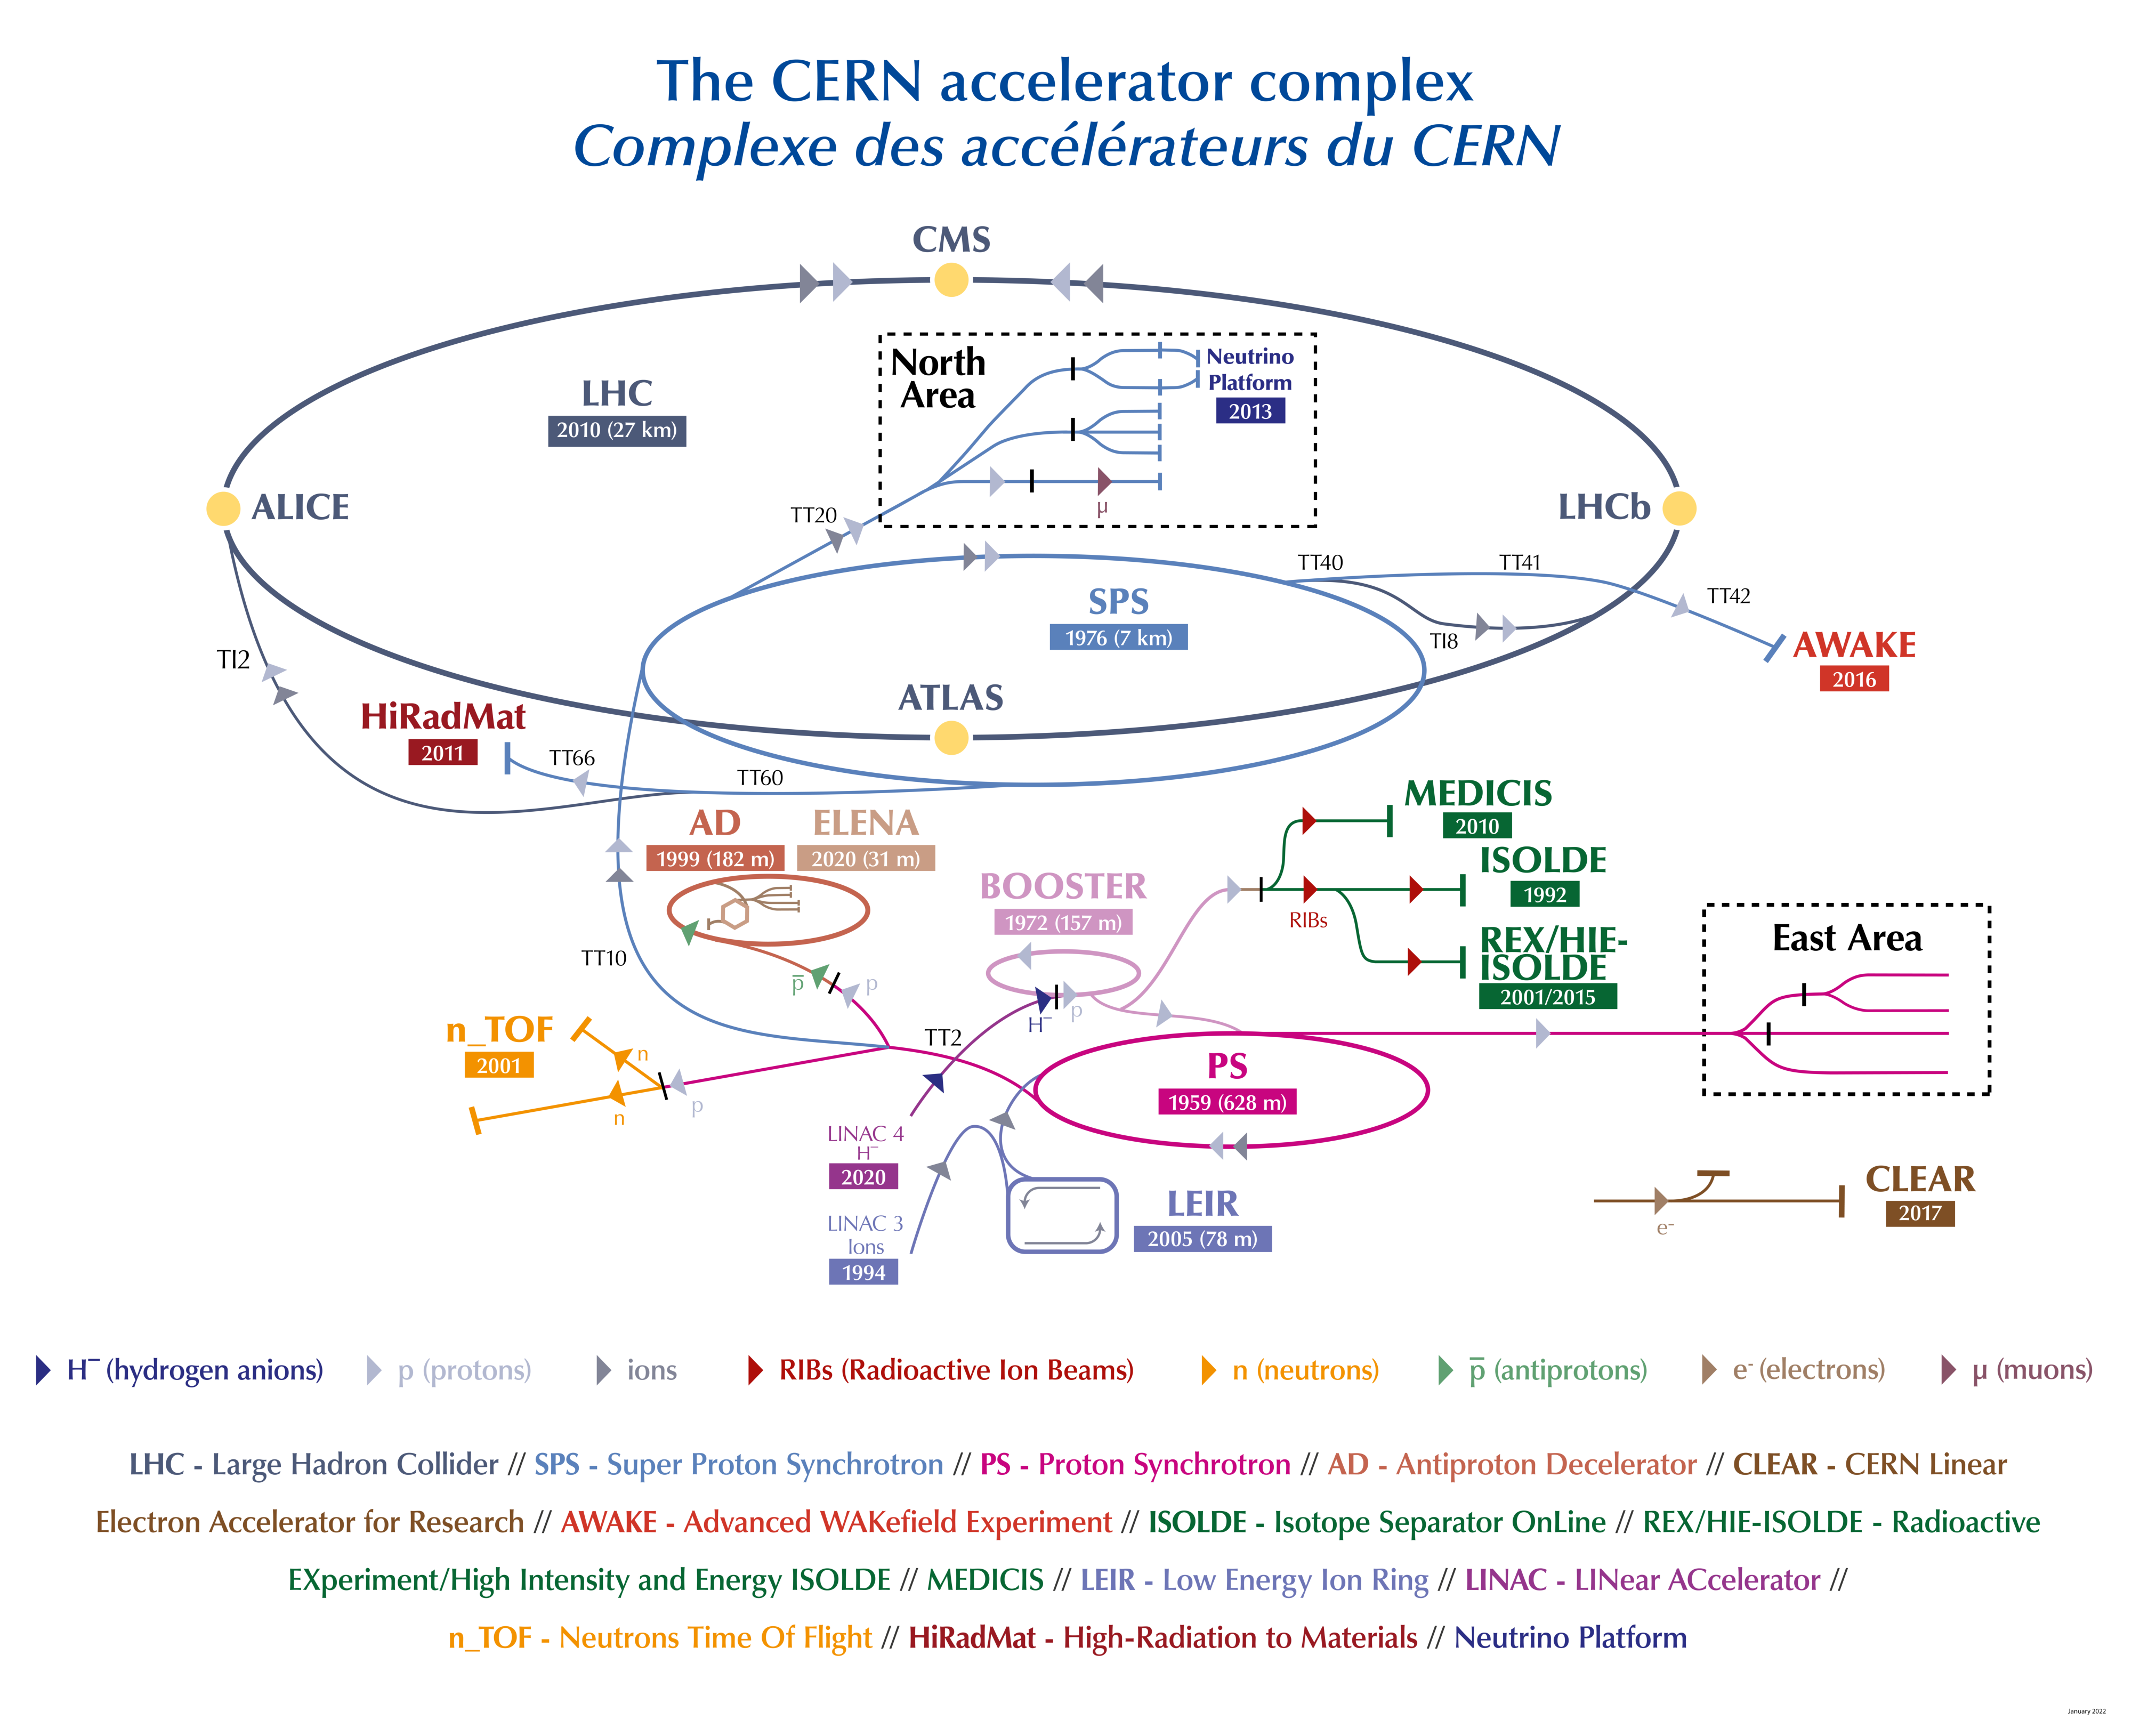
\includegraphics[width=0.8\linewidth]{figures/chapter_II/cern_complex.png}
    \caption{Schematic representation of the CERN accelerator complex.\cite{CERN-complex-2022}}
    \label{fig:cern_complex}
\end{figure}

La cadena comienza con una fuente de gas de hidrógeno, en la que se producen iones de hidrógeno negativos (H$^-$), formados por un protón y dos electrones. Los iones se extraen de la fuente con una energía de $45$ keV y se inyectan en el Linear accelerator (LINAC4), donde un cuadrupolo de radiofrecuencia (RFQ) agrupa los iones en paquetes de partículas y los acelera hasta 3 MeV, tras lo cual una serie de estructuras aceleradoras de radiofrecuencia elevan su energía hasta 160 MeV. A continuación, el haz se inyecta en el Proton Synchrotron Booster (PSB), un sincrotrón formado por cuatro anillos superpuestos, donde una lámina de carbono arranca los dos electrones de cada ion, de forma que a partir de este punto el haz está compuesto únicamente por protones. El PSB acelera los protones hasta 2 GeV antes de transferirlos a la siguiente etapa de la cadena.

Los protones se transfieren después al Proton Synchrotron (PS) donde alcanzan una energía de 26 GeV y donde se define la estructura temporal final del haz: mediante sucesivas divisiones de los paquetes de partículas, se forman trenes de paquetes (\textit{bunches}) separados por 25 ns, que es el espaciado con el que operará posteriormente el LHC. La última etapa previa al LHC es el Super Proton Synchrotron (SPS) que acumula varios trenes procedentes del PS y los acelera hasta 450 GeV, la energía de inyección del LHC.

Desde el SPS, los trenes se transfieren al LHC a través de dos líneas de transferencia independientes, cada una de las cuales llena uno de los dos anillos, de forma que los haces circulan en sentidos opuestos en tubos de vacío separados. Una vez se ha completado el número de paquetes previsto para cada haz, comienza la fase de aceleración gracias a cavidades superconductoras de radiofrecuencia que operan a $400$ MHz. Estas cavidades aportan a los protones del orden de $0.5$ MeV por vuelta y, al mismo tiempo, mantienen los paquetes confinados longitudinalmente. Así, a lo largo de unos veinte minuso, los haces alcanzan su energía final, que durante el Run 3 ha sido de $6.8$ TeV por haz, y una vez estabilizados se hacen colisionar en los cuatro puntos de interacción del anillo.

Estos puntos de intersección están instrumentados con particle detectors installed in underground caverns. "A Toroidal LHC ApparatuS" (ATLAS) and the "Compact Muon Solenoid" (CMS) experiments están situados en los dos diametrically opposite puntos del anillo, y reciben la mayor luminosidad instantánea de colisión. Son los dos general purpose experiments del LHC, diseñados para cubrir un programa de física muy amplio y en gran medida similar. The "LHC beauty" (LHCb) se centra en el estudio de CP-violation y de matter-antimatter asymmetry by studying b quarks physics. "A Large Ion Collider Experiment" (ALICE) is focused mostly on heavy ion collision and quark-gluon plasmas. 



\subsection{LHC Design and parameters}
\label{subsec:LHC_desing}
%
El LHC está instalado en el túnel de $26.7$ km de largo construido to host the LEP collider, por lo que su diseño está en gran parte condicionado por la reutilización de dicho túnel. El diámetro interior del túnel, de apenas $3.7$ m en los arcos, no deja espacio para anillos de imanes separados, por lo que el LHC adopta un diseño \textit{two-in-one}, en el que los dos tubos de vacío por los que circulan los haces en sentidos opuestos, cada uno con sus propias bobinas, se alojan en una misma estructura mecánica y en un mismo criostato.

La energía máxima que puede alcanzar un haz en un anillo de determinada circunferencia viene limitada por el campo magnético capaz de curvar su trayectoria. De esta forma, para mantener en órbita protones de $7$ TeV, el LHC emplea $1232$ dipolos superconductores capaces de generar un campo de $8.33$ T si se enfrían a $1.9$ K, temperatura que se consigue mediante helio superfluido~\cite{Bruning:2004ej}. Además de curvar la trayectoria, es necesario mantener el haz enfocado, para lo que se emplean $392$ cuadrupolos situados a lo largo de todo el anillo junto con imanes de órdenes multipolares superior que se encargan de corregir las imperfecciones del campo. El anillo se divide en ocho arcos, donde se sitúan los dipolos, y ocho secciones rectas, que albergan los puntos de interacción y los sistemas de aceleración, colimación y extracción del haz.

\label{sec:pp_pheno}
Aunque los dos haces de $7$ den lugar a colisiones con energía en el centro de masas de $\sqrt{s}=14$ TeV, la energía disponible para producir nuevas partículas realmente depende de la fracción $x$ delmomento del protón que porte cada uno de sus constituyentes, los partones —quarks y gluones. En consecuencia, la energía efectiva de la interacción es $\sqrt{\hat{s}}=\sqrt{x_1x_2\,s}$, que varía de un suceso a otro, de forma que el LHC explora simultáneamente un amplio rango de energías, y la producción de estados finales pesados, como un par de bosones de Higgs, solo es posible en la fracción de colisiones en que los partones portan una fracción de momento suficiente. El teorema de factorización permite separar la sección eficaz hadrónica QUE TIENE QUE VER AQUI LA SECCION EFICAZ? NO ESTAMOS HABLANDO DE ENERGÍAS? en una parte calculable perturbativamente, la sección eficaz partónica $\hat{\sigma}_{ij}$, y una parte no perturbativa, las funciones de distribución partónica (PDFs) $f_i(x,\mu_F)$, que describen la probabilidad de encontrar en el protón un partón $i$ con fracción de momento $x$~\cite{Collins:1989gx}:
\begin{equation}
    \sigma_{pp\to X} = \sum_{i,j}\int_0^1 dx_1\,dx_2\; f_i(x_1,\mu_F)\,f_j(x_2,\mu_F)\;\hat{\sigma}_{ij\to X}(x_1x_2\,s,\,\mu_R,\,\mu_F).
    \label{eq:factorization}
\end{equation}
Las PDFs no pueden calcularse a partir de primeros principios, sino que se extraen de ajustes globales a datos experimentales~\cite{NNPDF:2017mvq}. Por su parte, la escala de factorización $\mu_F$ y la de renormalización $\mu_R$ no son magnitudes físicas, sino consecuencia del truncamiento de la serie perturbativa, de forma que la dependencia del resultado con ellas refleja los órdenes no calculados. La variación de estas escalas, junto con la incertidumbre de las PDFs, constituye la principal fuente de incertidumbre teórica en la predicción de secciones eficaces, como las de producción de pares de bosones de Higgs discutidas en el Capítulo \ref{ch:theory}.


Dos haces de $7$ TeV dan lugar a colisiones con una energía en el centro de masas de $\sqrt{s}=14$ TeV, pero esta no es la energía disponible para producir nuevas partículas. Los protones no son partículas elementales, por lo que la interacción de interés no se produce entre los protones, sino entre sus constituyentes, los partones —quarks y gluones—, cada uno de los cuales porta una fracción $x$ del momento del protón. En consecuencia, la energía efectiva de la interacción es $\sqrt{\hat{s}}=\sqrt{x_1x_2\,s}$, que varía de un suceso a otro, de forma que el LHC explora simultáneamente un amplio rango de energías, y la producción de estados finales pesados, como un par de bosones de Higgs, solo es posible en la fracción de colisiones en que los partones portan una fracción de momento suficiente. El teorema de factorización permite separar la sección eficaz hadrónica en una parte calculable perturbativamente, la sección eficaz partónica $\hat{\sigma}_{ij}$, y una parte no perturbativa, las funciones de distribución partónica (PDFs) $f_i(x,\mu_F)$, que describen la probabilidad de encontrar en el protón un partón $i$ con fracción de momento $x$~\cite{Collins:1989gx}:

\\

%Los arcos están formados por celdas regulares en las que los dipolos se alternan con los cuadrupolos y los imanes correctores, mientras que las secciones rectas albergan los puntos de interacción y los sistemas de aceleración, colimación y extracción del haz, junto con los cuadrupolos que focalizan los haces antes de cada colisión~\cite{Evans:2008zzb}.

% Luminosidad
El alcance del LHC viene asimismo determinado por la luminosidad instantánea $\mathcal{L}$, que es el parámetro que relaciona el número de sucesos de un proceso dado que se producen por unidad de tiempo y su sección eficaz $\sigma$:
\begin{equation}
    \frac{dN}{dt} = \mathcal{L}\,\sigma .
    \label{eq:event_rate}
\end{equation}
Donde la $\mathcal{L}$ es una magnitud que depende únicamente de las condiciones de los haces. En el LHC, para haces de perfil gaussiano que colisionan con un ángulo de cruce, la luminosidad se expresa como
\begin{equation}
    \mathcal{L} = \frac{\gamma\, f_\text{rev}\, n_b\, N_b^2}{4\pi\, \varepsilon_n\, \beta^*}\, F, \qquad F = \left(1+\left(\frac{\theta_c\,\sigma_z}{2\sigma^*}\right)^2\right)^{-1/2},
    \label{eq:lumi}
\end{equation}
donde $\gamma$ es el factor relativista de los protones, $f_\text{rev}$ la frecuencia de revolución, $n_b$ el número de paquetes por haz, $N_b$ el número de protones por paquete, $\varepsilon_n$ la emitancia transversal normalizada y $\beta^*$ el valor de la función beta en el punto de interacción, que caracteriza el grado de focalización del haz. El factor $F$ da cuenta de la reducción geométrica debida al ángulo de cruce $\theta_c$, y depende del tamaño transversal $\sigma^*$ y longitudinal $\sigma_z$ de los paquetes. Los valores nominales de estos parámetros se recogen en la Tabla \ref{tab:lhc_parameters}.
%
\begin{table}[h!]
    \centering
    \begin{tabular}{l c c}
        \hline
        \textbf{Parameter} & \textbf{Symbol} & \textbf{Nominal value} \\
        \hline
        Beam energy & $E$ & 7 TeV \\
        Revolution frequency & $f_\text{rev}$ & 11.245 kHz \\
        Number of bunches per beam & $n_b$ & 2808 \\
        Protons per bunch & $N_b$ & $1.15\times10^{11}$ \\
        Normalized transverse emittance & $\varepsilon_n$ & 3.75 $\mu$m \\
        Beta function at the interaction point & $\beta^*$ & 0.55 m \\
        Transverse beam size at the interaction point & $\sigma^*$ & 16.7 $\mu$m \\
        Bunch length & $\sigma_z$ & 7.55 cm \\
        Crossing angle & $\theta_c$ & 285 $\mu$rad \\
        Geometric reduction factor & $F$ & 0.836 \\
        Instantaneous luminosity & $\mathcal{L}$ & $10^{34}$ cm$^{-2}$s$^{-1}$ \\
        \hline
    \end{tabular}
    \caption{Nominal LHC parameters for proton-proton collisions~\cite{Bruning:2004ej}.}
    \label{tab:lhc_parameters}
\end{table}

La Ecuación \ref{eq:lumi} muestra cuáles son las vías para aumentar la luminosidad. En primer lugar, la dependencia cuadrática con $N_b$ hace del número de protones por paquete el parámetro más efectivo, y este, junto con la emitancia, viene determinado por la cadena de inyección descrita en la Sección \ref{subsec:LHC_complex}. En segundo lugar, $\beta^*$ puede reducirse focalizando los haces justo antes del punto de interacción, función que desempeñan los cuadrupolos situados a ambos lados de cada experimento. Por último, el número de paquetes está limitado por el espaciado de $25$ ns. Sin embargo, con este espaciado los paquetes de ambos haces se encontrarían también en puntos distintos del de interacción, por lo que los haces deben cruzarse con un pequeño ángulo, lo que reduce la luminosidad a través del factor $F$.\\


Integrando la Ecuación \ref{eq:event_rate} en el tiempo, el número total de sucesos esperado para un proceso es $N=\sigma\int\mathcal{L}\,dt$. La luminosidad integrada, expresada habitualmente en fb$^{-1}$, es por tanto la magnitud que cuantifica el volumen de datos de un análisis, y su medida precisa es imprescindible para convertir un número de sucesos en una sección eficaz. En CMS, esta medida se realiza mediante detectores dedicados, denominados luminómetros, cuya respuesta se calibra en barridos de van der Meer, en los que los haces se desplazan uno respecto al otro para determinar su solapamiento~\cite{CMS:2021xjt}. La precisión alcanzada en cada uno de los años analizados en esta tesis, del orden del porcentaje, se detalla en la Sección \ref{sec:bbtt_systematics}.

% pileup
Sin embargo, con una luminosidad elevada no se produce una única interacción protón-protón por cada cruce de paquetes, sino varias simulaténas, de forma que el número medio de interacciones por cruce viene dado por:
\begin{equation}
    \mu = \frac{\mathcal{L}_b\,\sigma_\text{inel}}{f_\text{rev}},
    \label{eq:pileup}
\end{equation}
donde $\mathcal{L}_b$ es la luminosidad por paquete y $\sigma_\text{inel}$ la sección eficaz inelástica protón-protón. En condiciones nominales, $\mu$ es del orden de 25. Estas interacciones adicionales, conocidas como \textit{pile-up}, son en su inmensa mayoría procesos de baja transferencia de momento que se superponen a la interacción de interés, y a ellas se suman las procedentes de cruces anteriores y posteriores, cuya señal persiste en la electrónica del detector. Por tanto, el pile-up afecta a la reconstrucción de todos los objetos del suceso, y su mitigación constituye uno de los aspectos centrales de los algoritmos descritos en la Sección \ref{sec:POR}. La distribución de $\mu$ registrada por CMS durante el Run 3 se muestra en la Figura \ref{fig:pileup}.


\begin{figure}[h!]
    \centering
    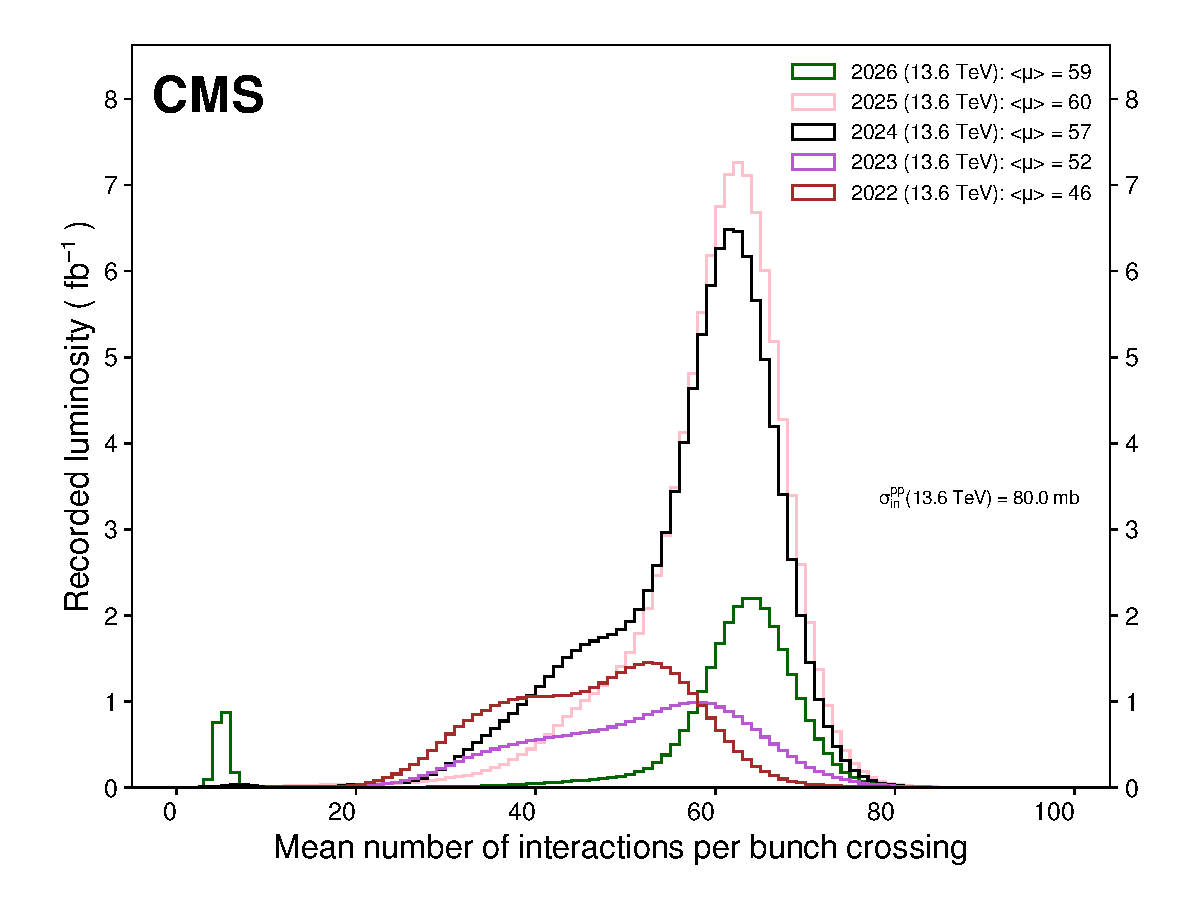
\includegraphics[width=0.75\linewidth]{figures/chapter_II/pileup_run3.pdf}
    \caption{Distribution of the mean number of interactions per bunch crossing recorded by CMS in proton-proton collisions during each year of Run 3, computed assuming an inelastic cross section of 80 mb~\cite{TOTEM:2017asr}. The mean value $\langle\mu\rangle$ of each year is indicated~\cite{CMS-LumiPublicResults}.}
    \label{fig:pileup}
\end{figure}






CIERRE DE LO QUE ME ABRE CADA PARAMETRO

The LHC is installed in a 26.7 km long tunnel built between 1984 and 1989 to host the
CERN Large Electron Positron (LEP) collider. The tunnel is located in the region nearby
Geneva and extends across the French and the Swiss borders. In the LHC, two separate,
counter-rotating particle beam lines are kept in orbit in two magnetic channels thanks to
44 Chapter 2. Experimental apparatus
the field generated by superconduting niobium-titanium coils. The particles are steered
by a magnetic field of 8.3T generated by a current of about 11 kA in the 1232 dipole
magnets, each measuring 15 metres of length and 35 tonnes of weight. The stability of
the beam dynamics is ensured by 392 quadrupoles magnets measuring 5 to 7 metres of
length, that focus the particles and keep them in a narrow beam. Special quadrupoles
are installed in front of the collision points to squeeze the beams and increase the proton
density in the collisions. Superconducting magnets are cooled with superfluid helium-4
and kept to a working temperature of 1.9K.

The LHC ring is made of eight 2.45km long arcs, where bending dipoles are placed, and
and eight 545m long straight sections. Because the tunnel is inherited from LEP, the
LHC design faces some space limitations: in the arcs, for instance, the tunnel has small
internal diameter of 3.7 m. Therefore, instead of implementing separate rings of magnets
for each of the beams, the two counter-rotating beamlines need to be hosted within a
single cryogenic and mechanic assembly; the antiparallel magnetic fields are generated
by two independent sets of coils, although they are are placed close enough to each other
that they are coupled both magnetically and mechanically.
The LHC electromagnets are made of copper-clad niobium-titanium superconductor,
amounting globally to about 470 tonnes. The beams are kept on their circular path
through the magnetic field of 1232 dipoles operating at 8.33 T, while 392 quadrupole
magnets keep the particles focused in narrow beams. Dedicated quadrupoles squeeze
the beams in proximity of the interaction points and magnets of higher multipole orders
correct smaller imperfections in the magnetic field. The operating temperature of the
magnets is 1.9 K (-271.25C); approximately 96 tonnes of superfluid helium-4 are needed
to keep them cool.

kept travelling in opposite directions before colliding in the designated
interaction points once they have reached a target energy; although the design center-ofmass
energy for proton-proton collisions is ps = 14TeV, the target energy of the LHC
acceleration stage changed over the research phases, as detailed in Sec. 2.1.4: 3.5TeV
until 2011, 4 TeV in 2012, 6.5 TeV from 2015 on.

Luminosity


\subsection{Operation}

The accelerator is a 27 km circular collider built around
100 m underground composed by two rings where two beams of protons or heavy
ions circulate in opposite directions inside vacuum pipes. The beams are bended
using 1232 superconducting dipoles, cooled down with super
uid helium to 1.9 K,
which generate an 8.3 T magnetic eld. To focus the beams and avoid spreading,
392 quadrupole magnets are used

The LHC is the last step of the accelerating chain in which the particles reach
the operating energies. The CERN accelerator complex is shown in Fig. 2.1. At the
beginning of the chain, hydrogen atoms are ionized and injected into the LINAC2,
where they are accelerated to an energy of around 50 MeV. Then, the beam is passed
through a series of circular synchrotrons, reaching 1.4 GeV after the BOOSTER,
26 GeV after the PS and 450 GeV after the SPS, before they enter into the LHC
and reach their target energy. The designed center-of-mass energy (ps) for protonproton
collisions is 14 TeV, although the target energy has changed over the different
phases: 7 TeV during 2010 and 8 TeV during 2011 and 2012 (3-year period called
Run 1), 13 TeV during Run 2 (2015-2018) and 13.6 TeV during Run 3 (which started
in 2022).

The accelerator complex at CERN is a succession of machines that accelerate particles to increasingly higher energies to uncover the mysteries of the Universe. Each machine or accelerator boosts the energy of a beam of particles, before injecting the beam into the next machine in the sequence. In the Large Hadron Collider (LHC) – dark blue line – particle beams are accelerated up to the record energy of 6.5 TeV per beam. Most of the other smaller accelerators in the chain have their own experimental halls where beams are used for experiments at lower energies.


Protons are progressively accelerated by Linac4 (purple), PS Booster (pink), PS (magenta), SPS (blue), and ultimately at the LHC (dark grey). The proton beams circulated through the LHC collide in the center of the four particle detectors (yellow dots): ATLAS, ALICE, CMS, and LHCb



- Schema CERN: accelerator complex (experiments)
- design parameters: luminosity
- operation and plan




\section{The CMS Experiment}
\label{sec:CMS}
\subsection{Coordinate system and proton-proton collision phenomenology}
%junto o por separado estas dos secciones?
\subsection{Detector structure (subdetectors)}
\subsection{CMS Trigger System}
\subsection{Data Acquisition and Computing systems}
%??? añadir esta subsection? o no me hace falta?






\section{CMS physics objects reconstruction}
\label{sec:POR}
\subsection{The Particle Flow algorithm}
\subsection{Final state particle reconstruction}
\label{subsec:Finalstate}
\subsection{Muon}
%... ver como me cuadra mas
\subsubsection{Muon}
\subsubsection{Hadronic \texorpdfstring{$\tau$}{τ} leptons}
\label{subsec:Taus}
\noindent The $\tau$-lepton is the heaviest lepton in the SM, with a mass of $1.777$ GeV. It is the only lepton that can decay both leptonically and hadronically, with a short lifetime of $2.9\times 10^{-13}$ s. Leptonic decays account for about $35\%$ of the $\tau$-lepton decay width, while hadronic decays account for approximately $64.8\%$, as shown in Table \ref{tab:tau_decays}, which reports the corresponding branching fractions. In all decays, neutrinos remain undetected, and it is not possible to measure the momentum of the decaying $\tau$ with exact precision.

\begin{table}[h!]
    \centering
    \begin{tabular}{l c}
        \hline
        \textbf{Decay Mode} & \textbf{BR (\%)} \\
        \hline
        \multicolumn{2}{l}{\textbf{Leptonic decays}} \\
        $\tau^- \to e^- \,\bar{\nu}_e\, \nu_\tau$ & 17.8 \\
        $\tau^- \to \mu^- \,\bar{\nu}_\mu\, \nu_\tau$ & 17.4 \\
        \hline
        \multicolumn{2}{l}{\textbf{Hadronic decays}} \\
        $\tau^- \to h^- \nu_\tau$ & 11.5 \\
        $\tau^- \to h^- \pi^0 \nu_\tau$ & 25.9 \\
        $\tau^- \to h^- \pi^0 \pi^0 \nu_\tau$ & 9.5 \\
        $\tau^- \to h^- h^+ h^- \nu_\tau$ & 9.8 \\
        $\tau^- \to h^- h^+ h^- \pi^0 \nu_\tau$ & 4.8 \\
        \textit{Other} & 3.3 \\
        \hline
    \end{tabular}
    \caption{Decay modes of the $\tau$ lepton and corresponding branching fractions (BR) in $\%$; the charged hadrons are denoted by h$^{\pm}$}
    \label{tab:tau_decays}
\end{table}


In the leptonic decay mode, the lepton is accompanied by two neutrinos and is reconstructed simply as the corresponding electron or muon following the standard procedures describes in the previous sections, along with the to neutrinos emitted along the $\tau$-lepton flight direction. While neutrinos do not leave a direct trace upon escaping the detector, they do generate a momentum imbalance in the transverse plane. By measuring the missing transverse momentum in the event, their presence can be inferred. Therefore, the main challenge in identifying such decays lies in reconstructing and measuring the missing transverse momentum (MET), which serves as an indirect measurement of neutrinos, as described in Section \ref{sec:MET}. In addition, the energy fraction of the decaying $\tau$-lepton carried by the electron or muon falls within a continuous spectrum, which makes it difficult to distinguish between leptonic $\tau$ decays and prompt leptons. These effects makes the identification and reconstruction of $\tau$ leptonic decay a particularly challenging task.

Nevertheless, since leptonic decays are reconstructed based on the corresponding light lepton, discussing the reconstruction of $\tau$ leptons implicitly refers to hadronic $\tau$ ($\tau_h$) reconstruction. Hadronic decay can occur either directly or via intermediate resonances such as $\rho$(770) or $a_1$(1260), resulting in a variety of charged and neutral hadrons. Due to charge conservation, the decay products include and odd number of charged hadrons, typically one or three, which are reconstructed as hadron jets and a neutrino $\nu_{\tau}$. Due to the high particle multiplicity in hadronic $\tau$ decays, a reliable reconstruction algorithm must be able to identify the PF candidates associated with the charged hadrons, as well as the photons originating from $\pi^0$ decay; group them to determine the decay mode; and determine the kinematic properties of the $\tau_h$. To meet these requirements, the reconstruction of hadronically decaying $\tau$ leptons is operated in CMS with the Hadron-Plus-Strips (HPS) algorithm {\color{red}[\ref{}]}.

The HPS algorithm is employed to identify and reconstruct $\tau_h$ candidates by verifying the compatibility of all PF jet candidates with a $\tau$-lepton. To this end, the HPS algorithm is seeded by the AK4 PF jet candidates reconstructed as in Section \ref{sec:Jet}, and for each seeding jet, all particles within a cone of radios $\Delta R<0.5$ around the jet axis are tested as hadron candidates or clusters of electron and photon candidates originating form neutral pions decays (photons from $\pi^0$ decays may convert into electron-positron pairs). These reconstructed objects are referred to as \textit{strips}, and their reconstruction is performed iteratively: candidates within the clustering region around each strip are progressively added, and the strip position is recomputed using a $p_T$-weighted average. The $\eta \times \varphi$ window is dynamically adjusted in each iteration to adapt to the strip $p_T$ and ensure optimal energy collection. This procedure is repeated until no further candidates are found. At this stage, the HPS algorithm combines both charged hadrons and strips inside the PF jet to form all the possible combinations of hadrons for the various decay modes (listed in Table \ref{tab:tau_decays}): h$^{\pm}$, h$^{\pm}\pi^0$, h$^{\pm}\pi^0\pi^0$, h$^{\pm}$h$^{\mp}$h$^{\pm}$ and h$^{\pm}$h$^{\mp}$h$^{\pm}\pi^0$ (plus the additional $\nu_{\tau}$). Each decay mode hypothesis includes additional quality and invariant mass requirements to ensure it aligns with a genuine $\tau_h$. Among all candidates within a seed region, the hadronic $\tau_h$ with the highest $p_T$ is selected.

One of the major challenges in the $\tau_h$ reconstruction lies in accurately distinguishing genuine $\tau$ leptons from misidentified objects, such as background events involving QCD multi-jet production. To enhance the purity of the hadronic $\tau$ reconstruction, a convolutional neural network (CNN), the \textsc{DeepTau} identification method {\color{red}[\ref{}]}, has been adopted in CMS analyses since the end of the LHC Run 2 as a tool to discriminate real $\tau_h$ from quark and gluon jets, as well as from electrons and muons. This machine learning (ML)-based algorithm integrates information from high-level reconstructed $\tau_h$ features, the decay mode extracted from the HPS algorithm and low-level data used to construct the PF candidates. The \textsc{DeepTau} algorithm defines three different discriminators, each targeting a specificy type of background: jets \textsc{DeepTauVSjet}, electrons \textsc{DeepTauVSe}, and muons \textsc{DeepTauVSmu}. Each discriminator has a different set of working points (WP). 

Although the origins of this identification method date back to Run 2, the \textsc{DeepTau} algorithm received major updates at the start of Run 3. This new version includes upgrades such as reducing discrepancies between data and simulation in regions of high hadronic purity by integrating domain adaptation techniques, and improving data handling, resulting in overall enhanced performance. The \textsc{DeepTau} algorithm has been shown to achieve a significant improvement in the identification and reconstruction of $\tau_h$ compared to previous algorithm. {\textcolor{red}{Figure illustrates this enhancement for the three discriminators.}}

For example, for a given jet rejection level, the efficiency for genuine tau h candidates is increased by 10–30%.

A further advancement in Run 3 pertains to boosted topologies. When $\tau$ leptons are produced by highly boosted resonances, their decay products become collimated within a narrow cone, often forming a single jet, similar to the behavior observed for AK8 jets. While no dedicated reconstruction existed in Run 2, an extension of the HPS algorithm has been developed for Run 3 to target high-momentum candidates by exploiting the jet substructure of the $\tau_h$ candidates. The algorithm reverses the final step in the clustering sequence that forms the large-radius jet to identify two sub-jets that are compatible with the expected topology of boosted $\tau$ decay. Specific requirements are in place to suppress misidentification with quark-gluon jets, electrons or muons. This approach has been shown to outperform the standard HPS for highly boosted $\tau$ leptons while maintaining optimal misidentification rates. The selected boosted $\tau$ candidates are then passed to the HPS algorithm for standard $\tau$ reconstruction.


Hadronically decaying tau leptons are key elements for analysis involving complex final states, such as the $HH\rightarrow bb\tau\tau$ analysis, where robust $\tau$ reconstruction plays a central role. Accurate and reliable reconstruction and identification of $\tau$ leptons are essential, as the performance of the algorithms described in this section directly impacts the sensitivity to such signatures. Therefore, their validation becomes a crucial component of this work, which will focus on a detailed assessment of the identification algorithms used in Run-3 and its performance across the 2022-2026 data-taking periods in Chapter \ref{ch:Tau}.







\section{Trigger???}
\label{sec:TRG}